\documentclass[11pt]{article}

% TODO
% [ ] Añadir algunas bases matematicas de lo que estamos haciendo
% [ ] Mirar el vídeo sobre la práctica para mirar si hay que añadir el codigo en la memoria

% Paquetes
%===============================================================================

% Paquete para incluir imagenes
\usepackage{graphicx}
\graphicspath{ {./Imagenes/} }

% Paquete para incluir trozos de codigo
\usepackage{listings}


% Metadatos del documento
%===============================================================================
\title{Práctica 1 - Memoria}
\author{Sergio Quijano Rey}
\date{\today}

% Separacion entre parrafos
\setlength{\parskip}{1em}


% Contenidos del documento
%===============================================================================

\begin{document}

% Portada del documento
\maketitle
\pagebreak

% Indice de contenidos
\tableofcontents
\pagebreak

% Primer ejercicio
\section{Ejercicio 1 - Búsqueda iterativa de óptimos}

% Apartado 1
\subsection{Apartado 1}

En este apartado se nos pide implementar el algoritmo de Grandiente Descendente. Esta función toma como parámetros de entrada:

\begin{itemize}
    \item \lstinline{starting_point}: punto inicial del que parte la búsqueda
    \item \lstinline{loss_function}: función de error que buscamos minimizar. En nuestro caso concreto, es una función real de dos variables
    \item \lstinline{gradient}: función vectorial 2-dimensional que representa el gradiente de \lstinline{loss_function}
    \item \lstinline{learning_rate}: la tasa de aprendizaje. Es el parámetro crítico, pues en esta sección nos centramos en estudiar el comportamiento del gradiente descendente en base a este parámetro (y también del starting\_point)
    \item \lstinline{max_iterations}: número máximo de iteraciones. Así tenemos una condición sufiente para saber que el algoritmo va a parar
    \item \lstinline{target_error}: error debajo del cual paramos de iterar
    \item \lstinline{verbose}: si es \lstinline{True}, la función devuelve el error de cada solución de las iteraciones
\end{itemize}

Esta función devuelve el vector de soluciones que hemos ido construyendo. Si queremos obtener la solución final, lo único que tenemos que hacer es acceder a la última posición. Así podemos generar las gráficas en las que plasmamos tanto la función de error como los puntos que vamos construyendo. También, si tenemos activado el parámetro Verbose, devolvemos el error en cada iteración, lo que es necesario para hacer las gráficas de evolución de error que se nos piden.

\subsection{Apartado 2}
\label{seccion:Apartado2}

Consideramos la función de error dada por:

\begin{displaymath}
    E(u, v) := (u^3 * e^{v-2} - 2v^2 e^{-u})^2
\end{displaymath}

Usar gradiente descendente para encontrar un mínimo de esta función, comenzando desde el punto $(u, v) = (1, 1)$ y
usando una tasa de aprendizaje $\eta = 0,1$.

Podemos mostrar la función de error en una vista de pájaro (la vista tridimensional solo será necesaria en casos en los que la vista de pájaro no sea suficiente). Preferimos esta vista bidimensional porque es más rápida de computar y en muchos casos más fácil de interpretar.

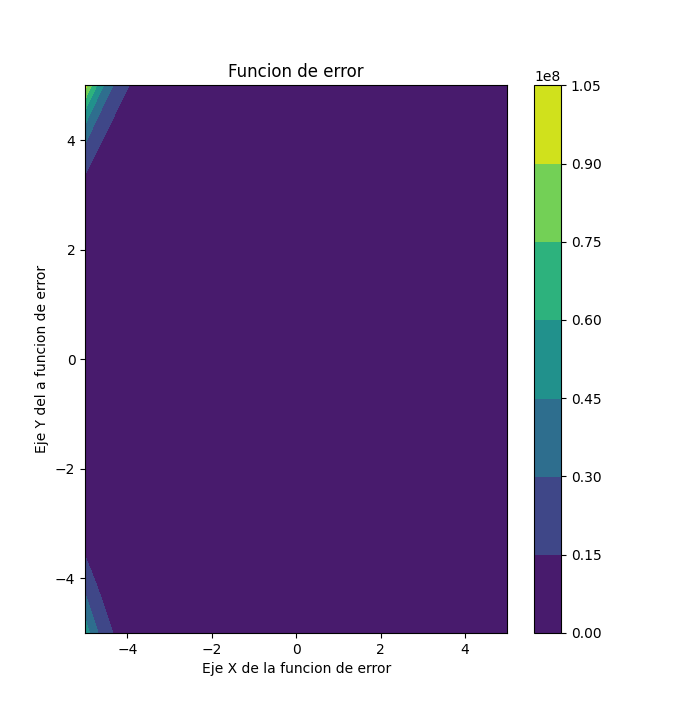
\includegraphics[scale=0.75]{FuncionErrorEjercicio1}

Los colores más azulados y oscuros indican los valores más bajos del error, mientras que valores verdosos y claros indican valores altos del error (la leyenda de la gráfica ya indica esto). Así que nuestros puntos deberán ir acercándose a zonas oscuras de la gráfica, si el comportamiento de los algoritmos es bueno.


\subsubsection{Subapartado a}

Calculamos analíticamente la expresión de las derivadas parciales:

\begin{displaymath}
    \frac{\partial E}{\partial u} = 2 * (u^3 * e^{v-2} - 2v^2 e^{-u}) * (3u^2 e^{v-2} + 2v^2 e^{-u}) \\
\end{displaymath}
\begin{displaymath}
    \frac{\partial E}{\partial v} = 2 * (u^3 * e^{v-2} - 2v^2 e^{-u}) * (u^3 * e^{v-2} - 4v e^{-u})  \\
\end{displaymath}
\begin{displaymath}
    \nabla E = (\frac{\partial E}{\partial u}, \frac{\partial E}{\partial v})
\end{displaymath}

Esta es la expresión del gradiente que usamos en el código. Expresión que mostramos por pantalla, como se indica en el guión de la práctica.

\subsubsection{Subapartados b y c}

Se manda explícitamente que usemos flotantes de 64 bits, para lo cual usamos la orden \lstinline{np.float64} para devolver todas nuestras funciones que representan los errores y las derivadas parciales.

Como se muestra en el código, solo necesitamos 10 iteraciones para quedarnos por debajo de un error (o valor de $E(u, v)$, que es lo que estamos considerando como función de error a minimizar) de valor $10^{-14}$. En el código indicamos que la primera iteración por debajo del error es la iteración 9, pero hay que tener en cuenta que empezamos a contar desde el cero.

Los resultados que mostramos por pantalla nos indican que alcanzamos la solución:

\begin{verbatim}
Numero de iteraciones: 10
Pesos encontrados: [1.15728885 0.91083837]
\end{verbatim}

Estos son los resultados vinculados a la onceava iteración (recordar que empezamos a contar desde el cero). Los resultados asociados a la décima iteración, en los que ya estamos por debajo del error buscado, son:

\begin{verbatim}
Primera iteracion por debajo de 10e-14: 9 (contando desde cero)
Las primeras coordenadas por debajo del error: [1.15728875 0.9108384 ]
\end{verbatim}

Todo esto se muestra en las salidas por pantalla de nuestro programa. Además, podemos mostrar cómo avanzan nuestras soluciones sobre la superficie que representa la función de error:

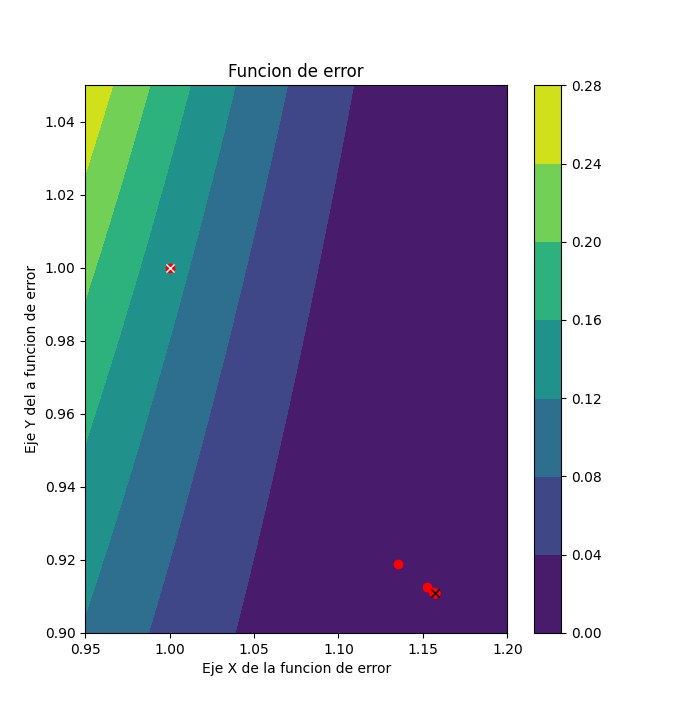
\includegraphics[scale=0.75]{EvolucionSoluciones01}

El punto con una cruz blanca es el punto inicial. El punto con una cruz negra es el punto final de la búsqueda. Viendo la gráfica de las soluciones generadas es claro que podríamos seguir avanzando con la búsqueda, pero decidimos parar porque estamos por debajo de la cota de error pedida.

La gráfica del error para los parámetros que se nos han indicado en ~\ref{seccion:Apartado2} es la siguiente:

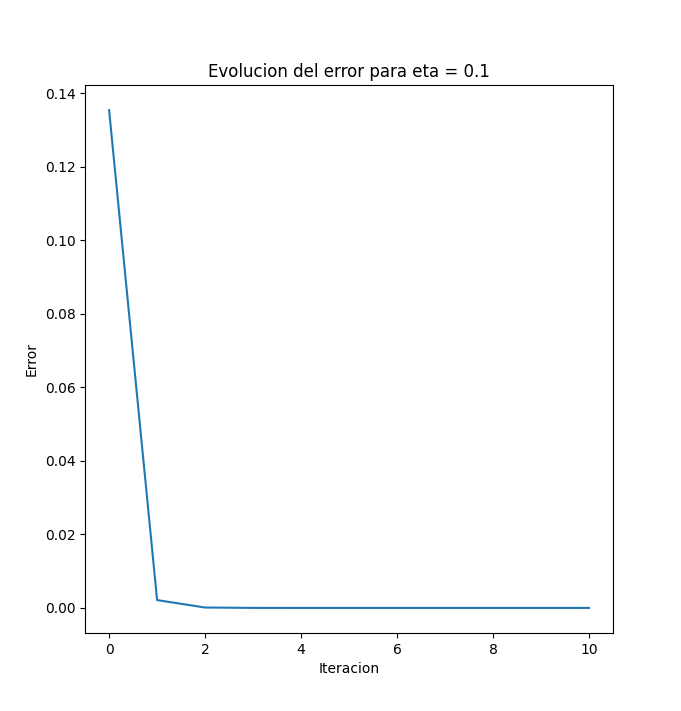
\includegraphics[scale=0.75]{EvolucionError01}

\subsection{Apartado 3}

Se considera ahora la función:

\begin{displaymath}
    f(x,y) := (x+2)^2 + 2(y-2)^2 + 2 sin(2\pi x) sin(2 \pi y)
\end{displaymath}

Como vamos a usar la técnica del gradiente descendente, necesitamos calcular analíticamente la expresión del gradiente:

\begin{displaymath}
    \frac{\partial f(x,y)}{\partial x} = 2(x+2) + 4 \pi sin(2 \pi y) cos(2 \pi x)
\end{displaymath}
\begin{displaymath}
    \frac{\partial f(x,y)}{\partial y} = 4(y - 2) + 4 \pi sin(2 \pi x) cos(2 \pi y)
\end{displaymath}
\begin{displaymath}
    \nabla f(x, y) = (\frac{\partial f(x,y)}{\partial x}, \frac{\partial f(x,y)}{\partial y})
\end{displaymath}

\subsubsection{Subapartado a}

Se nos pide usar gradiente descendiente para minimizar la función de error $f$. Además, se nos pide que usemos como parámetros del gradiente descendente:

\begin{itemize}
    \item $\eta = 0.01$
    \item $x_0 = -1, y_0 = 1$
    \item Máximo 50 iteraciones
\end{itemize}

Y que repitamos el experimento con un valor de $\eta = 0.1$.

Lo primero que hacemos es mostrar una gráfica en dos dimensiones de la función de error que queremos minimizar:

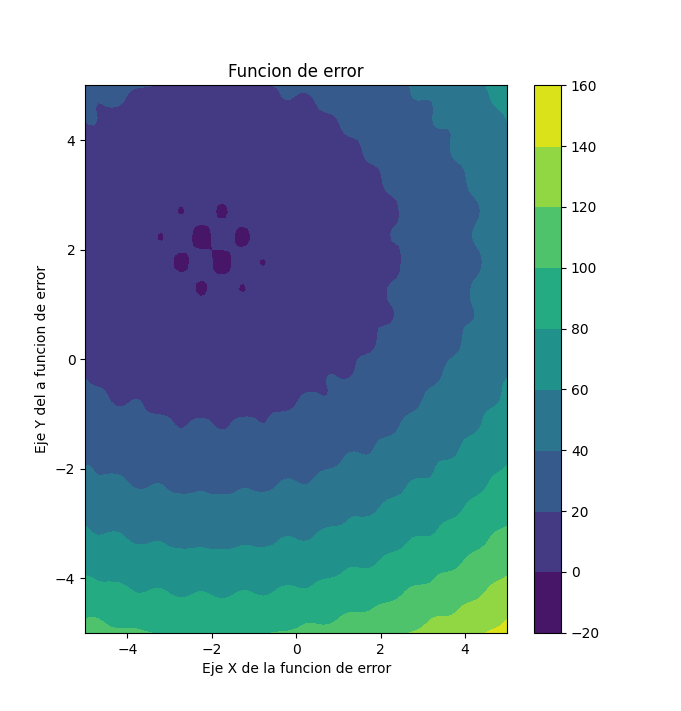
\includegraphics[scale=0.65]{FuncionErrorEjercicio1Apartado3}

Realizando gradiente descendente con los primeros parametros dados obtenemos la siguiente gráfica, en la que se muestra cómo evoluciona el valor del error según avanzan las iteraciones del algoritmo.

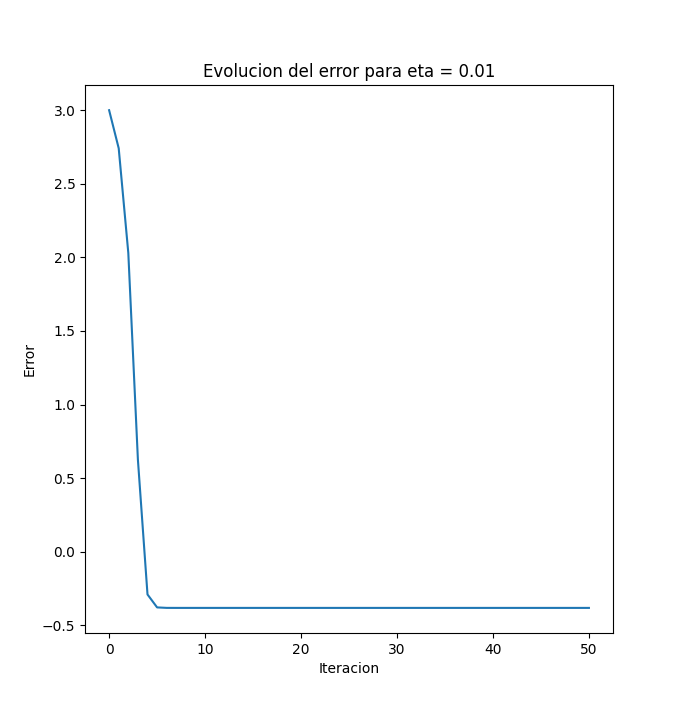
\includegraphics[scale=0.65]{EvolucionError02}

Mostramos, aunque no se nos pida en el guión, la traza del algritmo (soluciones plasmadas sobre la gráfica bidimensiona del error):

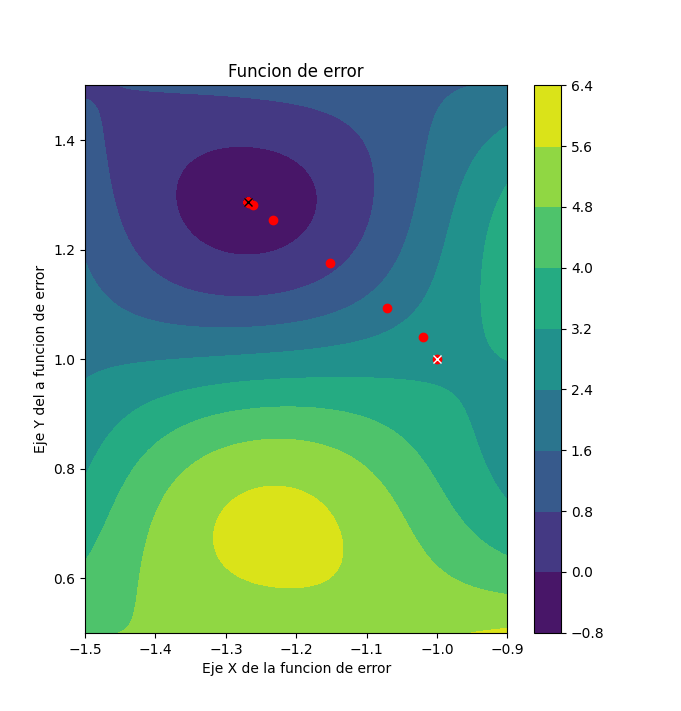
\includegraphics[scale=0.65]{EvolucionSoluciones02}

En esta gráfica se puede apreciar con facilidad que el algoritmo tiene el comportamiento deseado, pues cae con facilidad en un óptimo local.

Ahora realizamos el mismo proceso pero cambiando a $\eta = 0.1$. Obtenemos la siguiente gráfica de evolución del errolución del error:

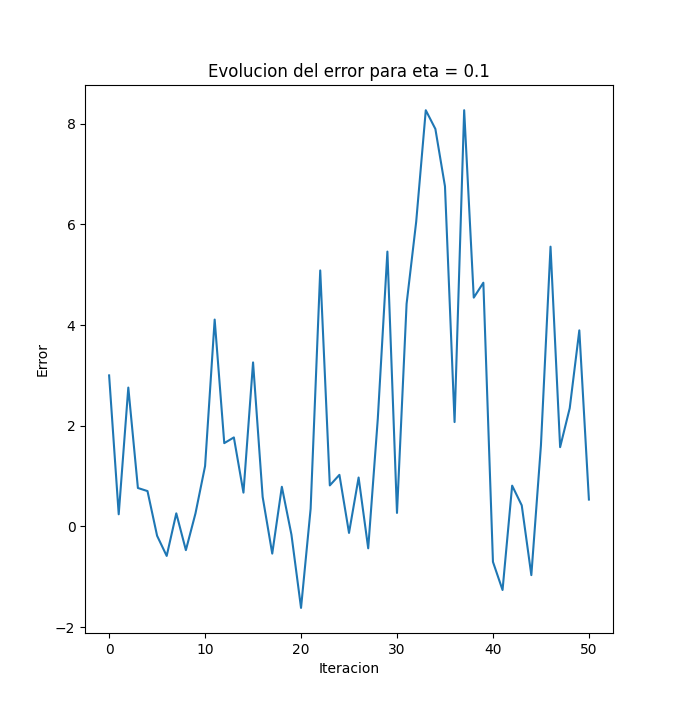
\includegraphics[scale=0.65]{EvolucionError03}

De esta gráfica ya podemos ver que el comportamiento del algoritmo no es el deseado. Lo que esperaríamos es que el error disminuyese monótamente en cada iteración. Sin embargo, lo que nos encontramos es con que el error oscila con grandes saltos. De lo estudiado en teoría, sabemos que el motivo sea seguramente un valor de $\eta$ demasiado grande. COn esto, cuando estamos cerca de una solución local, damos un salto muy grande en cierta dirección, saltando el óptimo local y yendo a una zona de alto error. Del mismo modo, de un salto desde una zona de alto error podemos acabar en una zona de muy bajo error. Es claro que este comportamiento errático no es deseable. Mostramos la traza de las soluciones en cada iteración para reforzar esta hipótesis sobre el mal comportamiento:

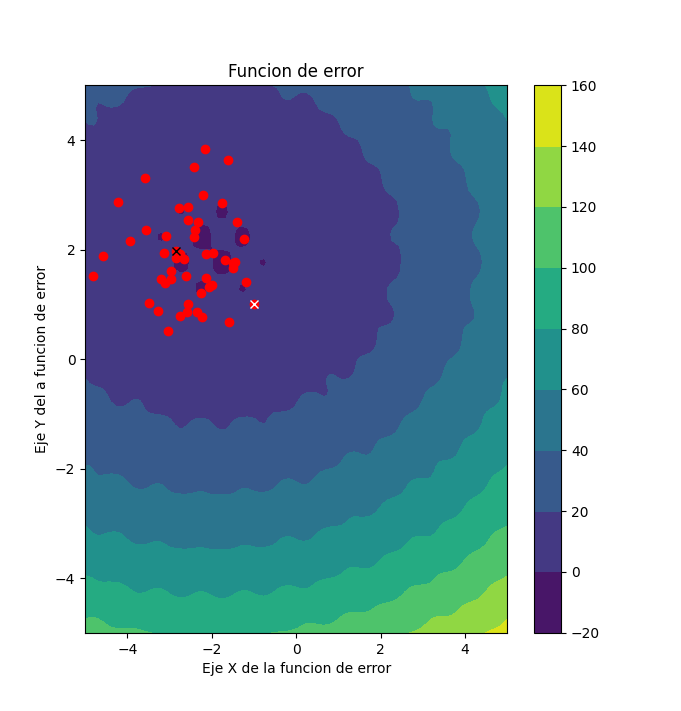
\includegraphics[scale=0.65]{EvolucionSoluciones03}

Con este gráfico, vemos que en la última iteración (del gráfico de evolución de error se deduce ya que se han consumido el total de iteraciones) hemos acabado, por buena suerte, en una buena zona de la función del error.

Con este ejemplo, podemos ver que es importante explorar con distintos valores de $\eta$, pues estos influyen mucho en el buen o mal comportamento del gradiente descendiente. Es más, ya podemos intuir que un ajuste dinámico del valor de $\eta$ puede ser muy interesante, pues como hemos visto en teoría, nos interesa avanzar con \emph{"pasos de gigante"} al principio con un $\eta$ grande, y disminuir el valor de $\eta$ al acercarnos a un óptimo local para tener más precisión en las iteraciones.

En estos dos ejemplos no muestro los valores numéricos de las soluciones obtenidas ni del error alcanzado. Considero que es mucho más interesante e informativo visualizar las gráficas, tanto del error como de la traza, pues estamos estudiando el comportamiento del algoritmo, no una solución concreta que no nos interesa al no ser un problema que realmente queramos resolver.

\subsubsection{Subapartado b}

Ahora repetiremos el mismo experimento pero tomando distintos valores para las soluciones iniciales. Y en este caso se pide que generemos una tabla con los valores obtenidos. Como no se especifica nada, tomamos $\eta \in {0.01, 0.1}$ y un máximo de 1000 iteraciones. Dejamos la cota de error a \lstinline{None} para que no se hagan comprobaciones de cotas. Además de la tabla, mostraremos las gráficas de la evolución del error y la traza de soluciones en los casos en los que sea interesante comentarlas (no en todas pues resultaría repetitivo).

La tabla con los datos generados es:

\begin{center}
    \begin{tabular}{| c | c | c | c |}
        Punto Inicial & Learning Rate $\eta$ & Solución alcanzada & Error Alcanzado \\
        \hline
        (-0.5, -0.5) & 0.01 & (-0.7934, -0.1259) & 9.1251\\
        (-0.5, -0.5) & 0.1 & (-1.1000, 3.4598) & 4.7785 \\
        (1, 1) & 0.01 & (0.6774, 1.2904) & 6.4375 \\
        (1, 1) & 0.1 & (-2.3820, 2.0917) & -0.5734 \\
        (2, 1) & 0.01 & (1.6466, 1.2954) & 12.7624 \\
        (2, 1) & 0.1 & (-1.8963,  2.1082) & 0.7969 \\
        (-2,  1) & 0.01 & (-2.2436,  1.2864) & -0.8685 \\
        (-2,  1) & 0.1 & (-0.8079, 2.0814) & 2.3492 \\
        (-3,  3) & 0.01 & (-2.7309,  2.7132) & -0.3812 \\
        (-3,  3) & 0.1 & (-2.1558,  3.0127) & 1.9427 \\
        (-2,  2) & 0.01 & (-2,  2) & $-4.7992 * 10^{-31}$ \\
        (-2,  2) & 0.1 & (-1.3420, 0.6155) & 5.3779 \\
        \hline
    \end{tabular}

\end{center}

Esta tabla ha sido obtenida a partir de los datos mostrados por pantalla. El programa no genera está tabla formateada, pero muestra por pantalla todos los valores que esta recoge.

\subsubsection{Comentarios sobre los resultados obtenidos}

Para los primeros valores de la tabla tenemos las siguientes dos gráficas:

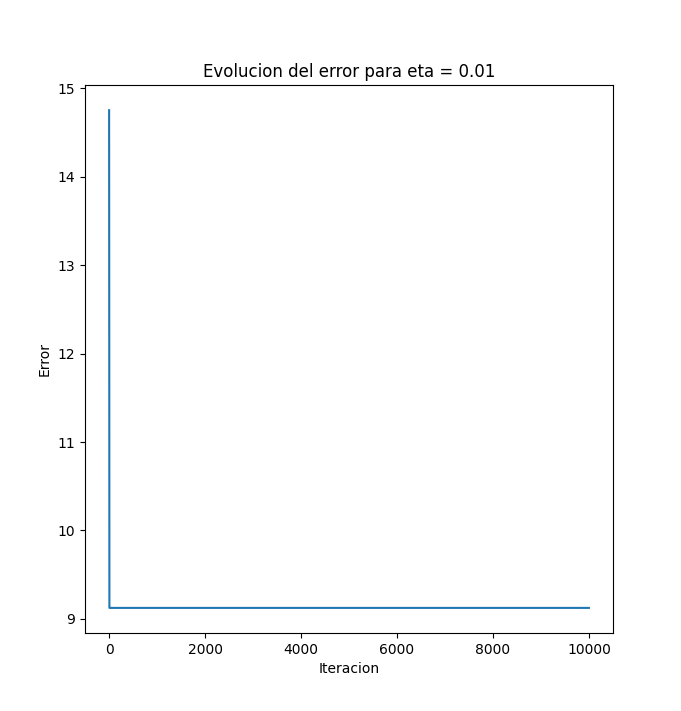
\includegraphics[scale=0.5]{EvolucionErrorExperimento01}

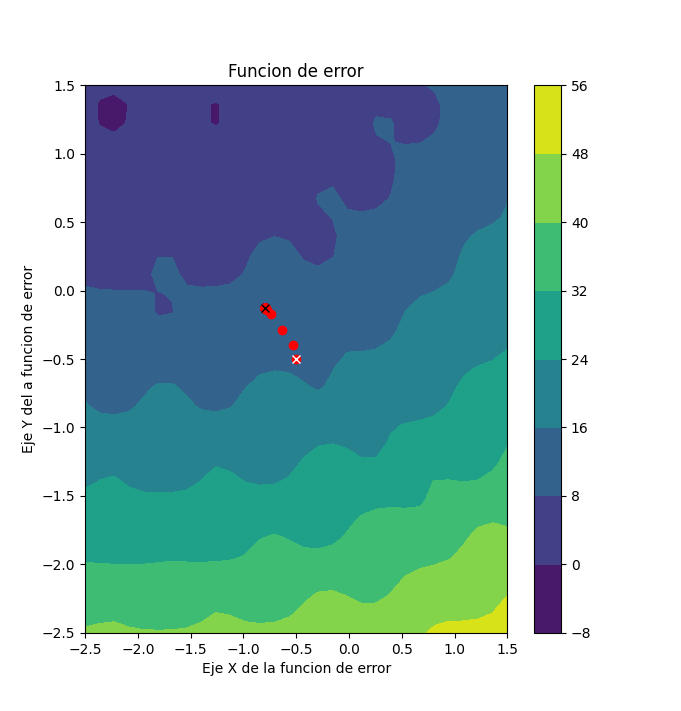
\includegraphics[scale=0.5]{EvolucionSolucionesExperimento01}

Vemos que damos un primer salto grande en el descenso del error, pero luego nuestro valor de $\eta$ es demasiado pequeño para converger a un óptimo local. La gráfica en tres dimensiones que generamos no aporta ninguna información de interés.

Para la segunda fila de la tabla, tenemos la siguiente gráfica de evolución del error:

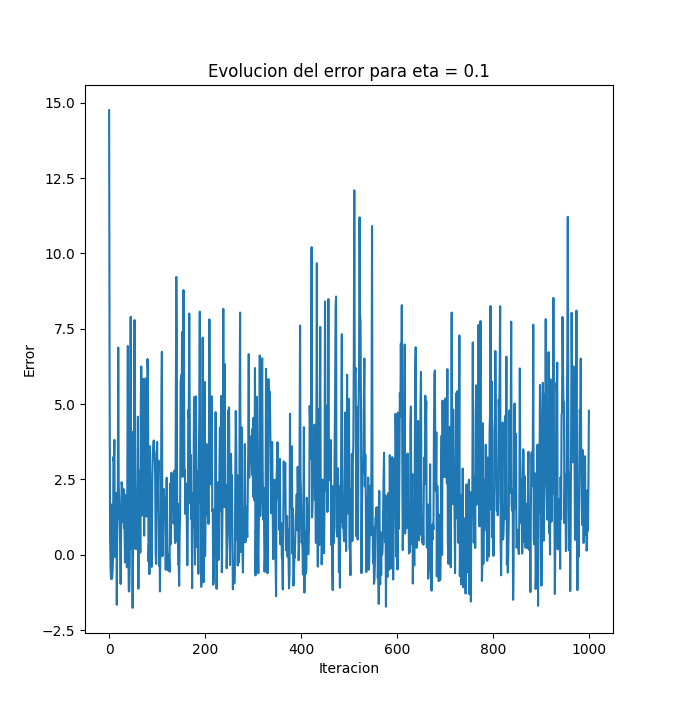
\includegraphics[scale=0.5]{EvolucionErrorExperimento02}

El valor de $\eta$ es demasiado grande, por lo tanto, el error fluctúa tanto. No es un valor apropiado para $\eta$, por lo que hemos comentado en apartados anteriores. Y a pesar de este comportamiento errático, por casualidad, acabamos con un error menor que con el valor apropiado para $\eta$ que aparece en la primera fila de la tabla.

Para la tercera fila de la tabla, parece que nos vuelve a pasar lo mismo que para la primera fila, a vista de las siguientes dos gráficas:

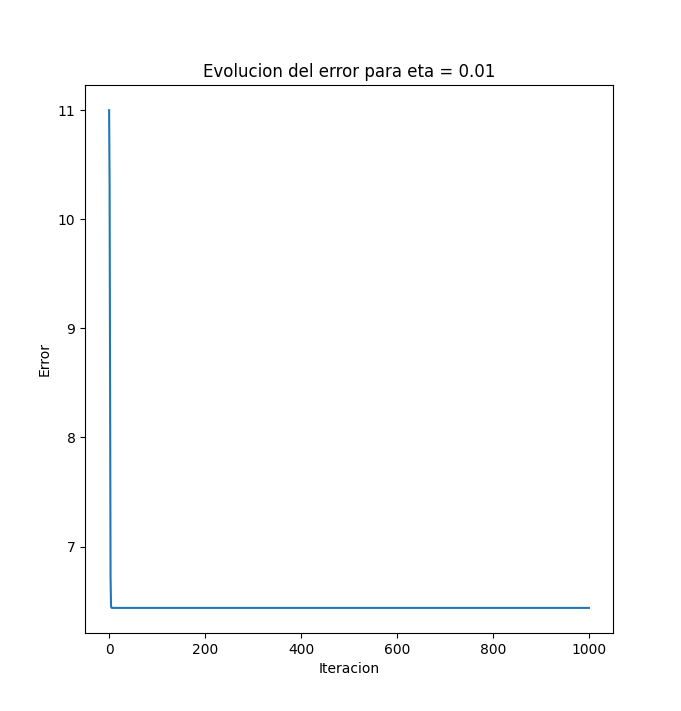
\includegraphics[scale=0.5]{EvolucionErrorExperimento03}

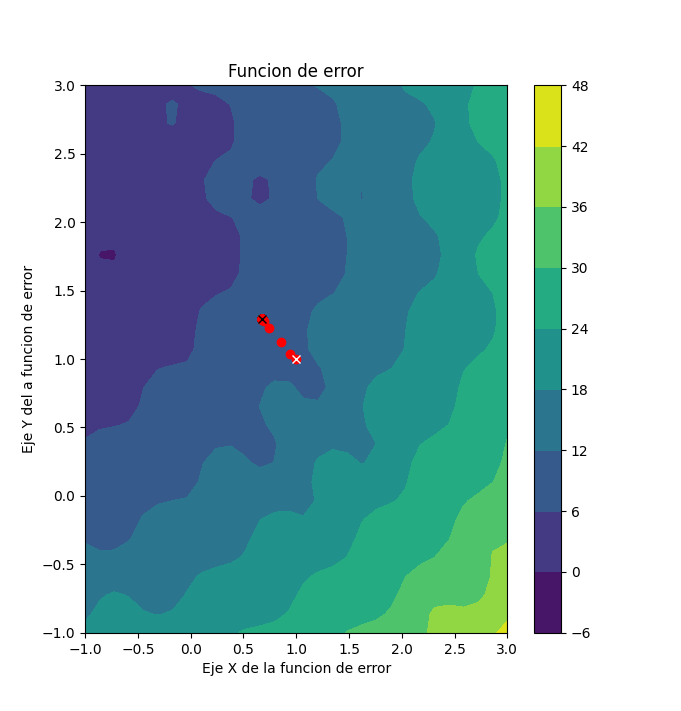
\includegraphics[scale=0.5]{EvolucionSolucionesExperimento03}

Pero si nos fijamos en la siguiente gráfica:

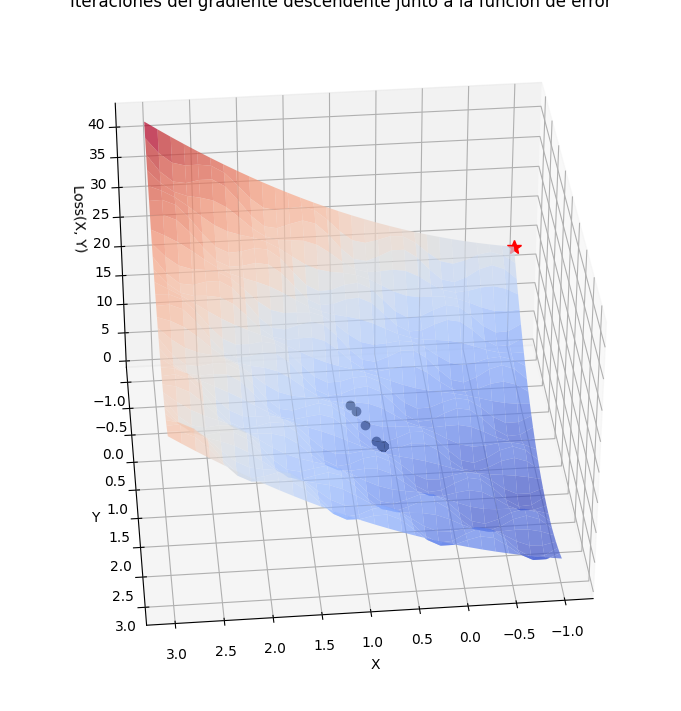
\includegraphics[scale=0.5]{Evolucion3dExperimento03}

Lo que podemos ver es que nos quedamos en una especie de \emph{bache} sobre el terreno. La conclusión es la misma, el valor de $\eta$ tan pequeño nos deja atascado, pero ahora es más claro el motivo. No es que simplemente los 1000 \emph{pasos} que damos sean muy cortos, es que llegamos a un óptimo local que con el pequeño valor de $\eta$ no conseguimos superar.

Para la cuarta fila, con un $\eta = 0.1$, tenemos un valor demasiado grande, lo que produce un comportamiento errático. Y de nuevo, por pura casualidad, alcanzamos un mejor valor de del error que usando un valor de $\eta$ adecuado. No incluyo gráficas pues son muy parecidas a las ya mostradas cuando ocurre esto, para evitar ser repetitivo.

Para la quinta fila, tenemos el mismo comportamiento comentado en el caso en el que las soluciones se quedaban atascadas en un \emph{bache}. Mientras que para la sexta fila volvemos a tener un comportamiento errático, que de nuevo, vuelve a dar mejores resultados por casualidad.

En la séptima fila, vemos como las soluciones convergen correctamente hacia un óptimo local para un valor de $\eta = 0.01$. Mientras que para $\eta = 0.1$, tenemos un comportamiento errático. Esto se muestra con claridad en las siguientes dos gráfica de la traza de las soluciones (en la leyenda se muestran los valores de \emph{eta})

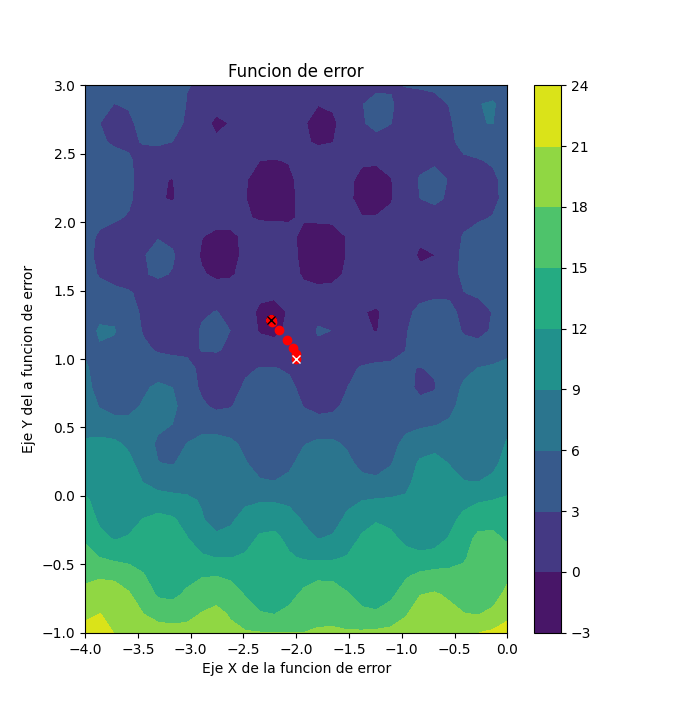
\includegraphics[scale=0.5]{EvolucionSolucionesExperimento07}

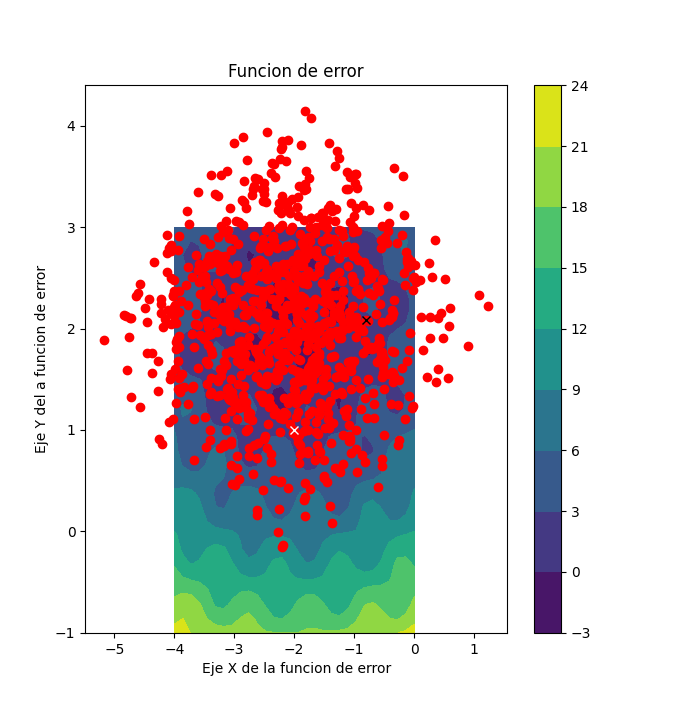
\includegraphics[scale=0.5]{EvolucionSolucionesExperimento08}

Además, en este caso, un valor apropiado de $\eta$ consigue mejores resultados que con un valor que produce comportamiento errático.

En la novena fila tenemos un muy buen comportamiento qeu da convergencia hacia un óptimo local (en la gráfica de la traza de la solución que muestra el programa esto se ve claramente. No añado esta gráfica pues ya se ha mostrado una muy parecida, para evitar ser repetitivo). Mientras que en la décima fila ($\eta$ demasiado grande) tenemos el claro caso de comportamiento errático, que en este caso produce peor solución que un adecuado valor de $\eta$.

En la undécima fila tenemos un comportamiento muy curioso. La solución inicial y final coinciden. Esto se ve claramente en las siguientes dos gráficas:

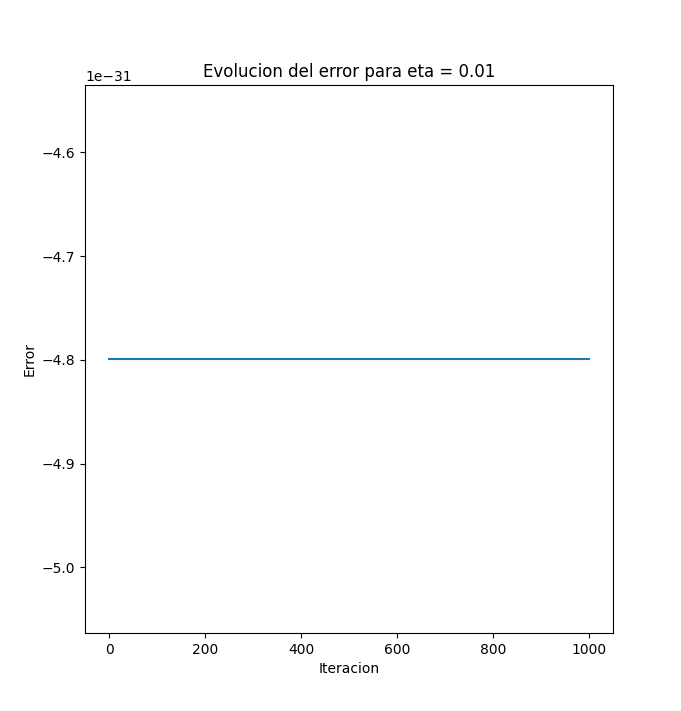
\includegraphics[scale=0.5]{EvolucionErrorExperimento11}

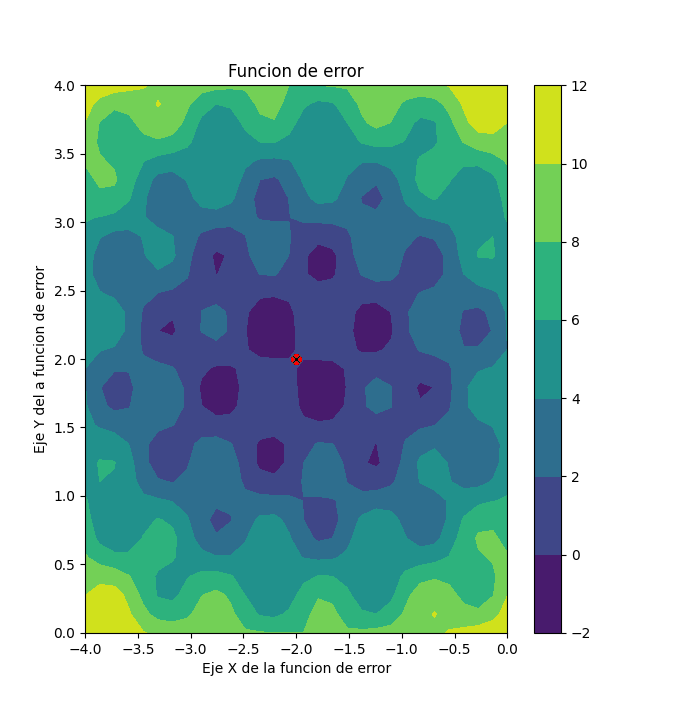
\includegraphics[scale=0.5]{EvolucionSolucionesExperimento11}

Vemos como estamos en el filo de dos \emph{agujeros} a los que nos interesaría caer. Estamos en un equilibrio muy inestable en lo que podría llamarse un punto de silla. En este caso en concreto, queremos que se rompa dicho equilibrio pues nos haría caer en uno de los dos óptimos locales. Notar también, que consumimos las mil iteraciones sin modificar la solución. Esto nos asegura que estamos en un punto de silla, pues el que no se mueva implica que el gradiente es cero. Gradiente nulo en un punto que no es óptimo indica con seguridad que es un punto de silla. Sin embargo, para un valor más grande de $\eta$ nos salimos del equilibrio, pero produciendo un comportamiento errático (como se muestra en la siguiente gráfica) que nos lleva a una peor solución:

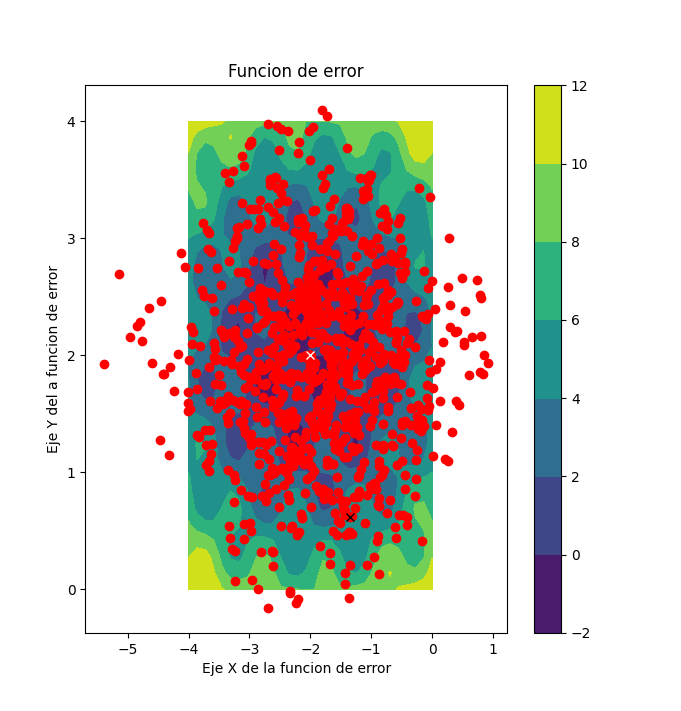
\includegraphics[scale=0.5]{EvolucionSolucionesExperimento12}

\subsection{Apartado 4}

La búsqueda de un mínimo global de una función arbitraria presenta varias dificultades, como hemos podido comprobar en estos casoss de estudio.

Para comenzar, no conocemos a priori si la función estudiada tiene un mínimo global. Tenemos resultados como el que nos asegura qque en una función convexa, todo mínimo local es un mínimo global (análogo con funciones cóncavas y máximos).

Los métodos analíticos para calcular puntos críticos son poco útiles en la práctica en espacios paramétricos de gran dimensionalidad. O con funciones para las que no existen soluciones analíticas, a pesar de que las funciones que definen el problema sean suficientemente regulares (continuas, diferenciables, $C^\infty$, $\ldots$), con lo que estas deben ser aproximadas por métodos numéricos. Por tanto, para muchos casos de uso, estas técnicas no van a ser factibles.

Y en otros muchos casos, vamos a trabajar con funciones de error que directamente no van a ser analíticamente tratables, por lo que quedan directamente descartados estos métodos analíticos. Es aquí donde entran en juego otros métodos, como búsquedas heurísticas o el método del gradiente descendente (que en este caso, se apoya en una propiedad analitica como es la existencia del gradiente).

Este método en concreto, que es el que estudiamos en este apartado, tiene las problemáticas usuales de los métodos iterativos para la búsqueda de óptimos locales. Dependen de parámetros como la solución inicial escogida, condiciones de parada, tamaño de la población de búsqueda (en caso de las técnicas vistas hasta ahora, solo tenemos una solución en la población de soluciones sobre las que realizamos la búsqueda).

Pero en el caso concreto del gradiente descendente, dependemos de forma crítica de elegir un valor adecuado para $\eta$, pues tendrá un gran impacto a la hora de decidir si la búsqueda del óptimo local tiene un comportamiento bueno (descenso del error monótono a un buen ritmo) o un mal comportamiento (evolución del error no monótono, con grandes picos, a un ritmo elevado, o por otro lado, descenso monótono pero a un ritmo demasiado lento, lo que hace que se atasque en malos óptimos o que no consiga llegar al óptimo local al agotar las iteraciones máximas permitidas).

La elección de este valor de $\eta$ además depende en gran medida de la función de error que queremos minimizar, y el valor de la solución de la que parte la búsqueda iterativa. Por tanto, y como ya se ha comentado, sería interesante disponer de técnicas para ajustar de forma dinámica el valor del \emph{learning\_rate}, pues nos interesa tener un valor alto al inicio para alejarnos rápidamente de zonas de alto error, y descender el valor de $\eta$ para tener más precisión a la hora de acercarnos al óptimo local. Y todo esto, en cada caso concreto con el que nos encontremos (hasta ahora, dependiendo de la solución inicial y de la función concreta que estemos minimizando).

Además, en las dos funciones de error estudiadas, hemos tenido que calcular analíticamente la expresión del gradiente para poder operar. Aunque esto no debería ser un gran problema con otras funciones, puesto que existen paquetes de cálculo simbólico como \lstinline{sympy} o aproximaciones numéricas del gradiente en un punto (como por ejemplo, diferencias finitas).

\pagebreak

\section{Ejercicio 2 - Regresión Lineal}

\subsection{Descripción del problema}

Buscamos ajustar modelos de regresión a vectores de características extraídos de imágenes de dígitos manuscritos. Estas características son:

\begin{itemize}
    \item Intensidad: valor medio del nivel de gris
    \item Simetría: respecto al eje vertical
\end{itemize}

Solo trabajaremos con los dígitos 1 y 5.

Cargaremos los datos, tanto de entrenamiento como de testing, de ficheros dados por los profesores de prácticas. La función que usamos para leer los datos, \lstinline{readData}, también ha sido dada por los profesores.

Es importante tener en cuenta que la matriz de datos que cargamos del fichero ya tiene una primera columna de unos. Esta columna es necesaria porque representa el sumando del término independiente en las ecuaciones lineales con las que estamos trabajando de forma matricial. De no ser así, tendríamos que añadir esta columna de unos para poder operar cómodamente con la matriz. En el experimento con características no lineales, añadimos columnas a la matriz con la orden \lstinline{np.insert(X, nueva_columna)}

Además, en este ejercicio, usaremos regresión lineal con la intención de clasificar los datos. Es decir, para un dato de entrada, devolvemos una solución real en un intervalo dado (regresión lineal). Después, tomamos como valor de clasificación la etiqueta cuyo valor numérico está más cercana a nuestra predicción de regresión. En el caso concreto de este ejercicio, las etiquetas son -1 y 1, luego es suficiente con quedarnos con el signo de la predicción de la regresión como valor de clasificación.

\subsection{Apartado 1}

Se nos pide estimar un modelo lineal a partir de los datos proporcionados, usando tanto el algoritmo de la pseudo-inversa como el algoritmo de gradiente descendente estocástico. Las etiquetas de los datos serán:

\begin{itemize}
    \item 1: para los dígitos cinco
    \item -1: para los dígitos uno
\end{itemize}

Una vez cargados los datos, estos pueden ser visualizados en un \emph{scatter plot}:

\begin{center}
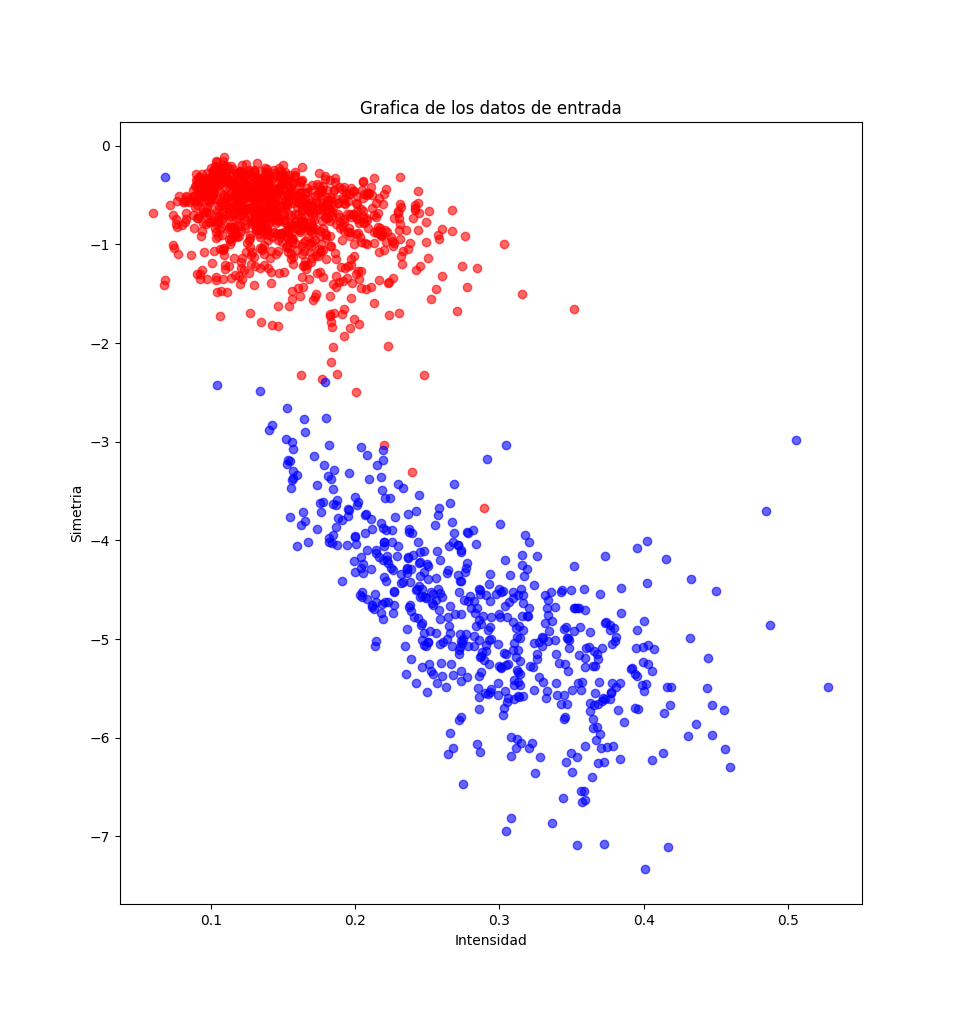
\includegraphics[scale=0.45]{NubeDatosOriginales}
\end{center}

Los puntos azules se corresponden con los unos, mientras que los rojos se corresponden con los cincos. Además, añadimos transparencias a los puntos para que sean más apreciables las zonas en las que hay mas concentración de puntos.

\subsubsection{Pseudo-Inversa}

Los resultados que mostramos por pantalla una vez ejecutado el algoritmo de la pseudo-inversa es:

\begin{lstlisting}
Los pesos obtenidos son: [-1.11588016 -1.24859546 -0.49753165]
El error de clasficacion en la muestra Ein es: 2.2408193670794097
El error de clasificacion fuera de la muestra Eout es: 2.439522584578059
El error cuadratico medio en la muestra Ein es: 0.07918658628900388
El error cuadratico medio fuera de la muestra Eout es: 0.13095383720052575
El error porcentual en la muestra Ein es: 0.5124919923126201%
El error porcentual fuera de la muestra Eout es: 1.650943396226415%
\end{lstlisting}

Este algoritmo calcula una solución cerrada en un paso, pues está usando el despeje matemático del sistema de ecuaciones que se nos plantea. Así que así hemos calculado la mejor solución, la que menor error va a cometer, al menos en los datos de entrenamiento y con el error cuadrático medio.

El error porcentual obtenido es muy bueno, tanto en la muestra de entrenamiento (un $0.5125\%$) como en la muestra de testing (un 1.6509\%). Como al usar la pseudo-inversa obtenemos la mejor solución, la información que esto nos aporta es que los datos con los que estamos trabajando están altamente correlados de forma lineal.

El error cuadrático es menos interpretable que el porcentual, pues depende de la escala de los datos con los que estemos trabajando, con las unidades en las que estemos trabajando\ldots. Además, al ser una media de suma de errores al cuadrado es más complicado que lo interpretemos sin tener otras referencias. Este error cuadrático medio nos servirá para hacer comparaciones con los errores cuadráticos de los métodos iterativos, pues como ya se ha mencionado, la pseudo-inversa obtiene el error mínimo para este problema, al menos para el error cuadrático medio. Y también es interesante tener un control sobre el error cuadrático medio pues es la función de error que los métodos iterativos van a tratar de minimizar (de nuevo, este algoritmo no es un método iterativo, da una solución cerrada en un paso).

El error de clasificación es el error que aparece en la teoría, en el contexto del algoritmo \emph{PLA}. El profesor ya nos comentó que estos métodos serán tratados en la siguiente práctica, pero hemos pensado que no vendría mal tener una referencia sobre esa medida de error.

Un inconveniente de este algoritmo es que para matrices mucho más grande que esta, es más lento que métodos iterativos como los que vamos a explorar a continuación.

Ahora mostramos la recta que separa los datos en los dos grupos en los que clasificamos. Es lo que podríamos llamar la recta frontera de la clasificación. Un dato lo clasificamos de una u otra forma según el signo de la predicción, por tanto, la frontera de clasificación será la recta que prediga los datos a un valor de cero, y con ello hacemos el siguiente desarrollo:

\begin{displaymath}
y = w_0 + w_1 x_1 + w_2 x_2
\end{displaymath}

La frontera será por tanto los valores para los que tengamos la predicción $y = 0$ y por tanto:

\begin{displaymath}
    0 = w_0 + w_1 x_1 + w_2 x_2 \Longrightarrow x_2 = \frac{1}{w_2} (-w_0 - w_1 x_1)
\end{displaymath}

y con esta fórmula ya podemos representar la recta frontera:

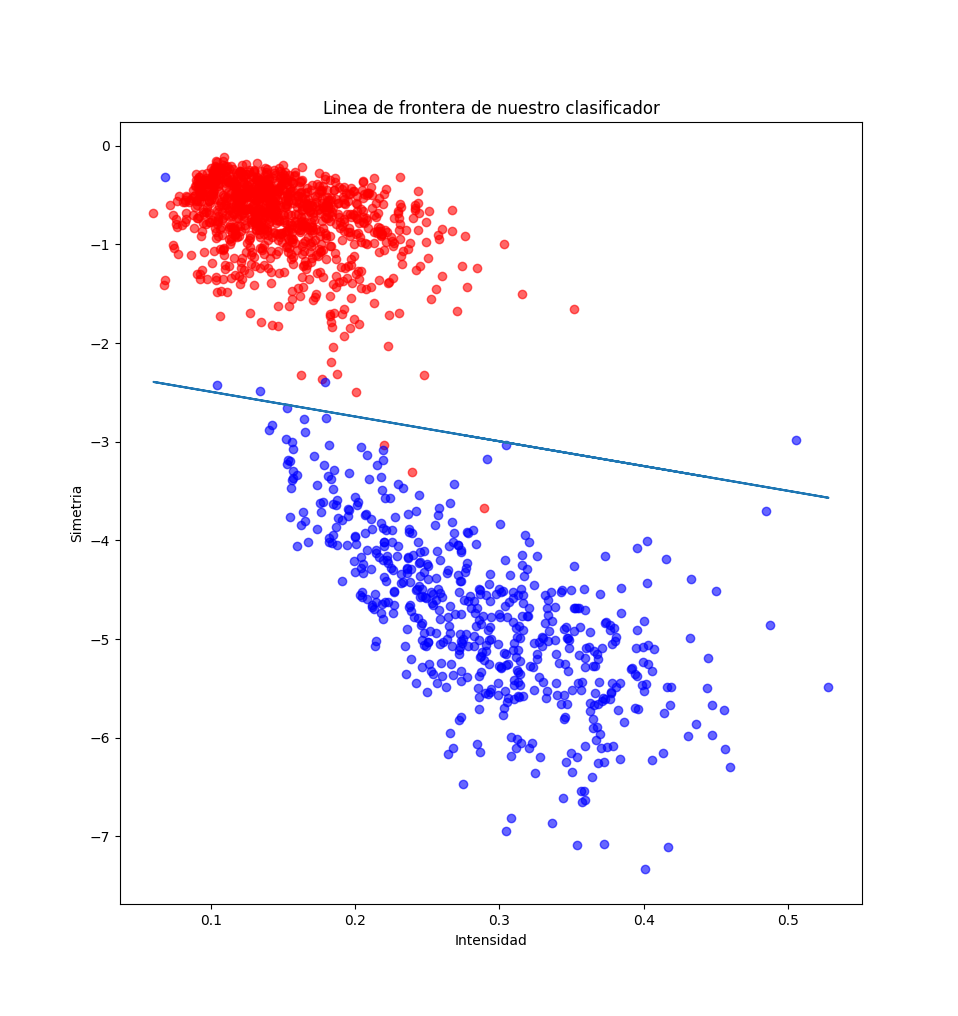
\includegraphics[scale=0.55]{FrontierLine01}

Esta recta frontera está representada con los datos de entrenamiento en el fondo. Además de esta gráfica, voy a mostrar una gráfica para ver dónde fallamos. En esta gráfica, los datos bien clasificados se mostrarán en gris, mientras que los datos mal clasificados se mostrarán en rojo. Dicha gráfica sobre los datos de entrenamiento es:

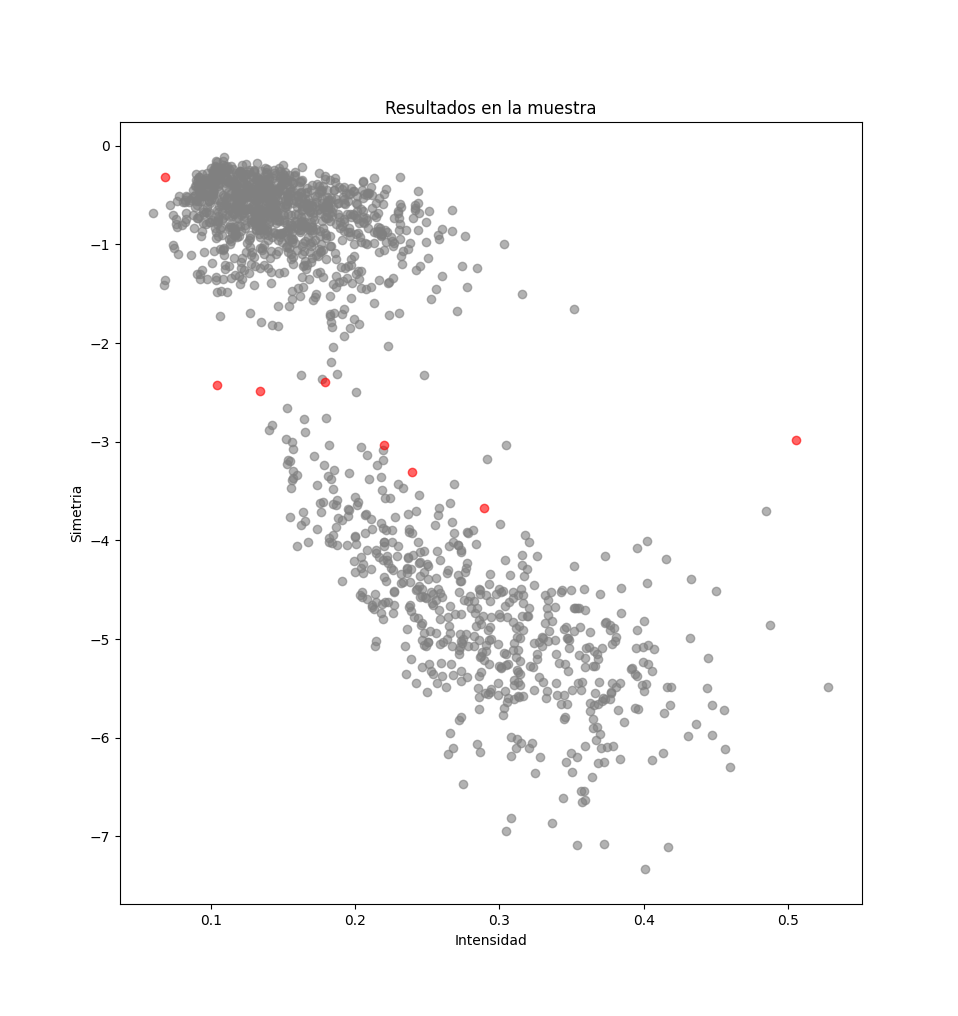
\includegraphics[scale=0.55]{BadPoints01}

Y la misma gráfica sobre los datos de test es:

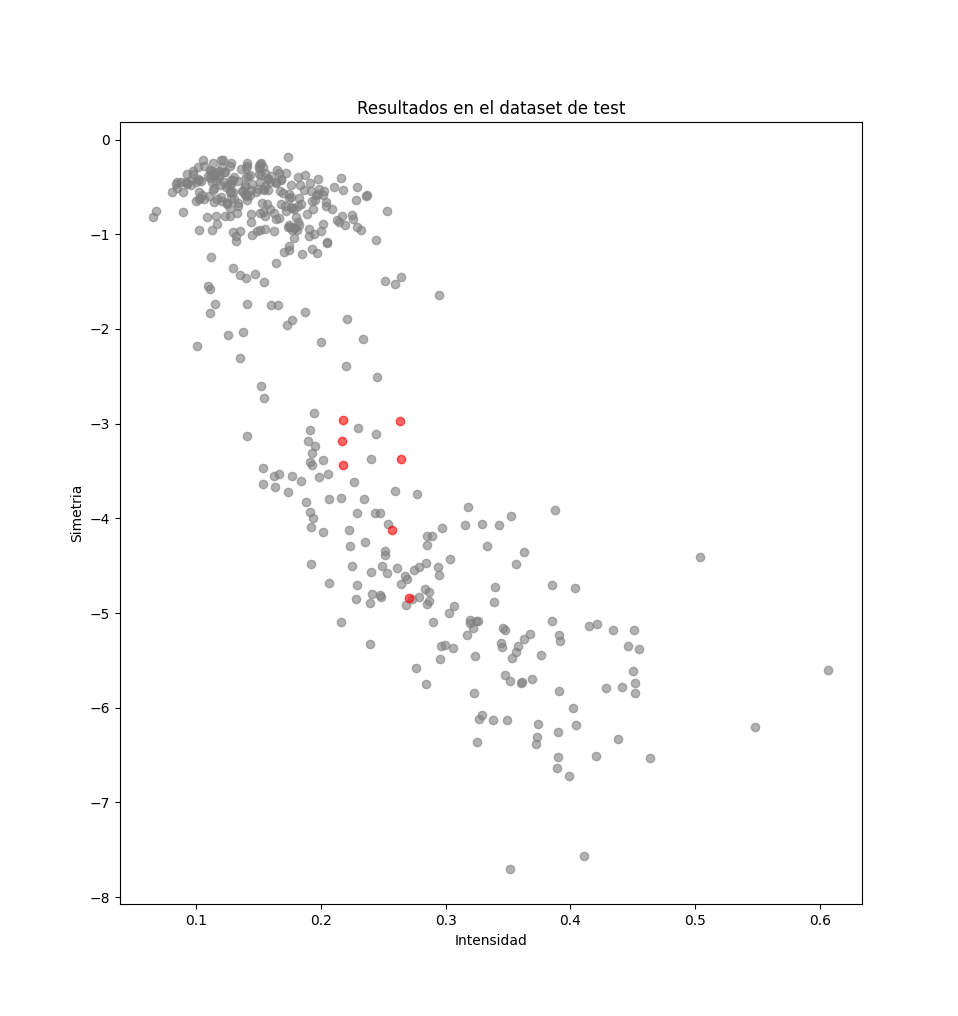
\includegraphics[scale=0.55]{BadPoints02}

Por tanto, podemos concluir que la muestra de datos está bien correlada linealmente y por tanto esta técnica tiene buenos resultados, a vista de los resultados reflejados en \lstinline{E_in} y \lstinline{E_out}. Además como no tenemos una gran cantidad de datos, el algoritmo devuelve la solución en un tiempo razonable.

\subsubsection{Stochastic Gradient Descent}

Este algoritmo depende de generar valores aleatorios. Así que, para trabajar con resultados reproducibles, fijamos la semilla aleatoria con \lstinline{np.random.seed(123456789)}.

Stochastic Gradient Descent, en su formulación clásica, trabaja con \lstinline{batch size = 1}, pero como nos indica el profesor de prácticas, es mejor explorar distintos valores de \emph{batch size}, así que realmente estamos trabajando con \emph{MiniBatch Stochastic Gradient Descent}.

Probaremos con un $batch\_size \in \{1, 32, data\_size\}$, donde $data\_size$ es el tamaño de la matriz de datos, con lo que tenemos, segun el valor del $batch\_size$:

\begin{itemize}
    \item 1: Stochastic Gradient Descent clásico
    \item 32: Minibatch con un valor del $batch\_size$ convencional
    \item 64: Minibatch con otro valor del $batch\_size$ convencional
    \item $data\_size$: Batch Gradient Descent, algoritmo que hemos usado en el Ejercicio 1
\end{itemize}

En estas pruebas solo nos quedaremos con los errores porcentuales, al ser los más fácilmente interpretables, y una vez escogido el tamaño del $batch\_size$, mostraremos los resultados completos. Además, siguiendo la indicación de nuestro profesor de prácticas, con 200 iteraciones sobre los minibatches generados, debería ser suficiente. Por otro lado, el valor del \emph{learning rate} lo dejaremos a $0.01$ tras haber hecho una exploración de posibles valores. Esta exploración no la incluimos también por no hacer demasiado extensa la memoria de esta práctica.

\begin{center}
    \begin{tabular}{| c | c | c | c |}
        Tamaño del minibatch & Error Porcentual en la muestra & Error porcentual fuera de la muestra \\
        \hline
        1 & 0.4484 \% & 1.8867\% \\
        32 & 0.4484\% & 1.6509\% \\
        64 & 0.4484\% & 1.6509\% \\
        $data\_size$ & 0.4484\% & 1.6509 \\
        \hline
    \end{tabular}
\end{center}

Todos los algoritmos corren en poco tiempo, salvo cuando usamos $data\_size$, que tarda algo más. Todos los errores, cuando miramos cuatro cifras decimales, son los mismos, salvo cuando usamos $batch\_size = 1$, que fuera de la muestra obtiene peores resultados. Por tanto, decido quedarme con $batch\_size = 32$, por se un valor bastante convencional, que produce buenos resultados y que tarda poco.

Así que corriendo el algoritmo con un valor de $batch\_size = 32$ obtenemos los siguientes resultados que mostramos por pantalla:

\begin{lstlisting}
Los pesos obtenidos son: [-1.0312233  -0.11892069 -0.40199688]
El error de clasficacion en la muestra Ein es: 1.959996706581955
El error de clasificacion fuera de la muestra Eout es: 2.5841736601550416
El error cuadratico medio en la muestra Ein es: 0.10448833536429288
El error cuadratico medio fuera de la muestra Eout es: 0.1533263011697918
El error porcentual en la muestra Ein es: 0.4484304932735426%
El error porcentual fuera de la muestra Eout es: 1.650943396226415%
\end{lstlisting}

Tanto fuera como dentro de la muestra, obtenemos errores porcentuales por debajo de los errores porcentuales de los errores porcentuales del algoritmo de la pseudo-inversa. Esto puede ocurrir al estar minimizando el error cuadrático medio y no un error porcentual. Sin embargo, el error cuadrático medio es más alto con este algoritmo que con la pseudo-inversa, lo que era de esperar.

El error porcentual solo tiene en cuenta si clasificamos bien un punto o no. Mientras que el error cuadrático medio mide también cómo de lejos está la predicción a través de regresión del valor de la etiqueta que queremos alcanzar. Por ejemplo, podemos predecir para un dato de entrada con verdadera etiqueta 1 la salida 0.57. Respecto al error porcentual, no estamos cometiendo error, pues la clasificación que se deriva es correcta. Pero para el error cuadrático medio se incluye en la sumatoria de la media un sumando $(1 - 0.57)^2$.

Mostramos la recta frontera obtenida con este algoritmo:

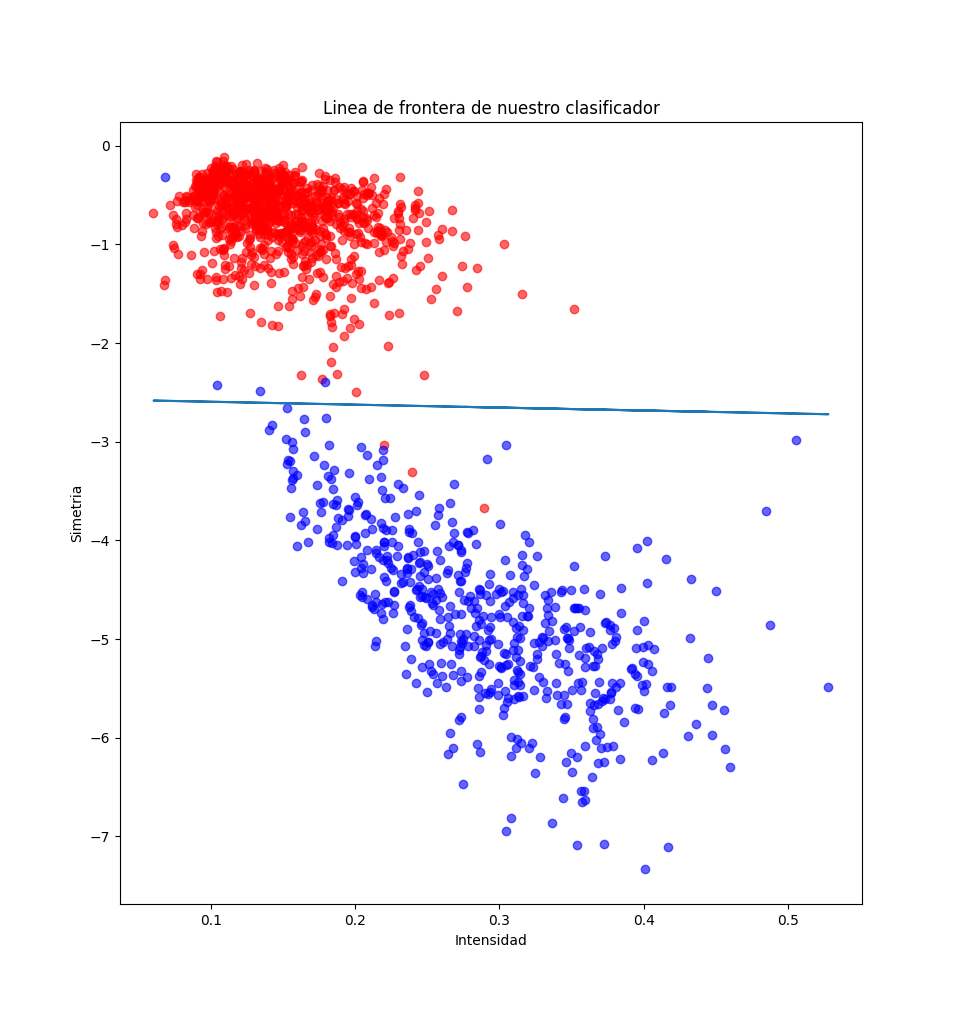
\includegraphics[scale=0.55]{FrontierLine02}

También mostramos las gráficas de puntos errados, tanto en la muestra de entrenamiento como en la muestra de test:

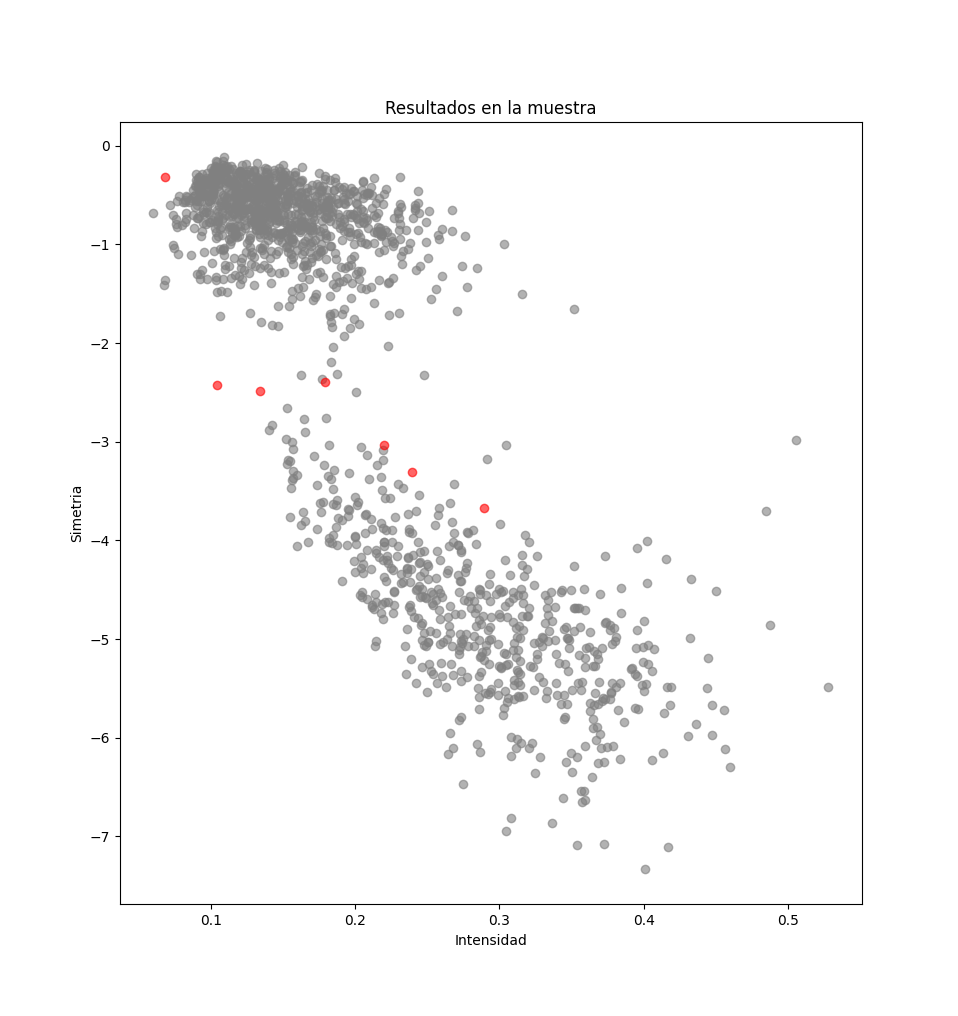
\includegraphics[scale=0.55]{BadPoints03}

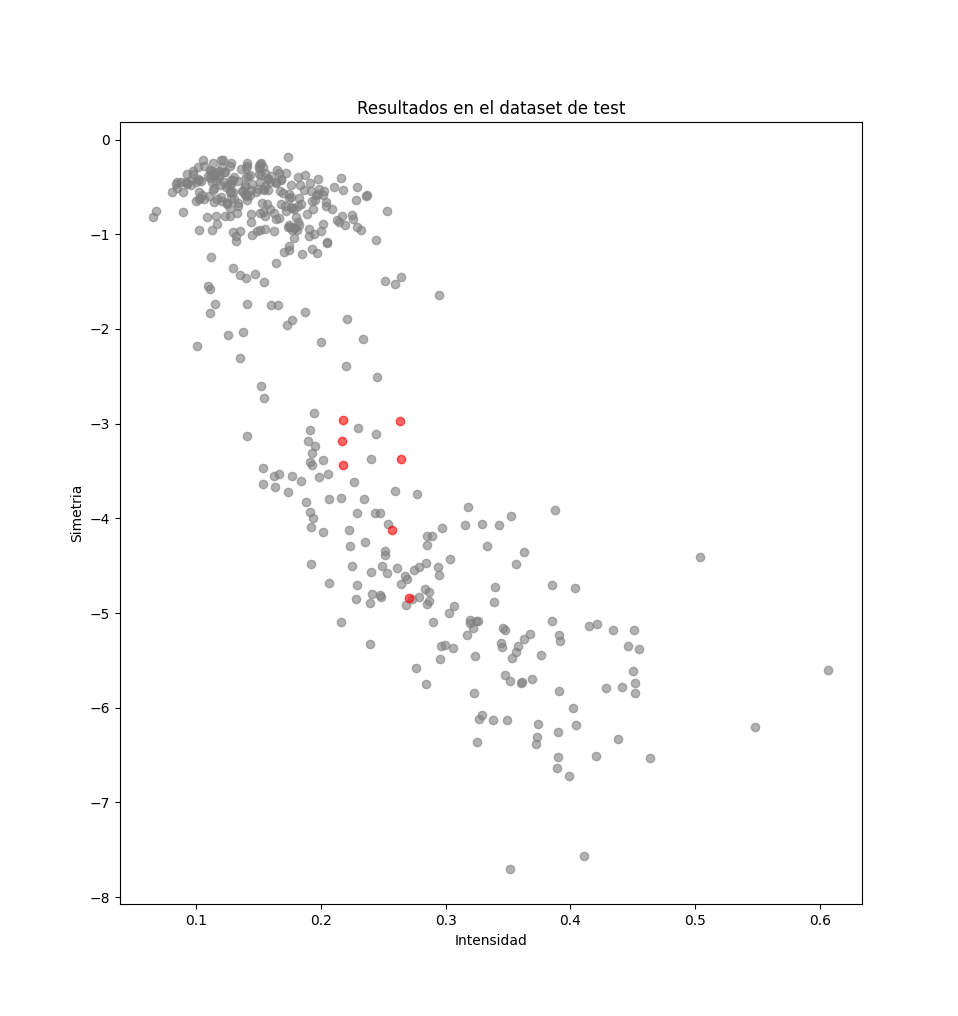
\includegraphics[scale=0.55]{BadPoints04}

Al estar usando un proceso iterativo, podemos mostrar cómo avanza el error en cada iteración sobre cada uno de los minibatches:

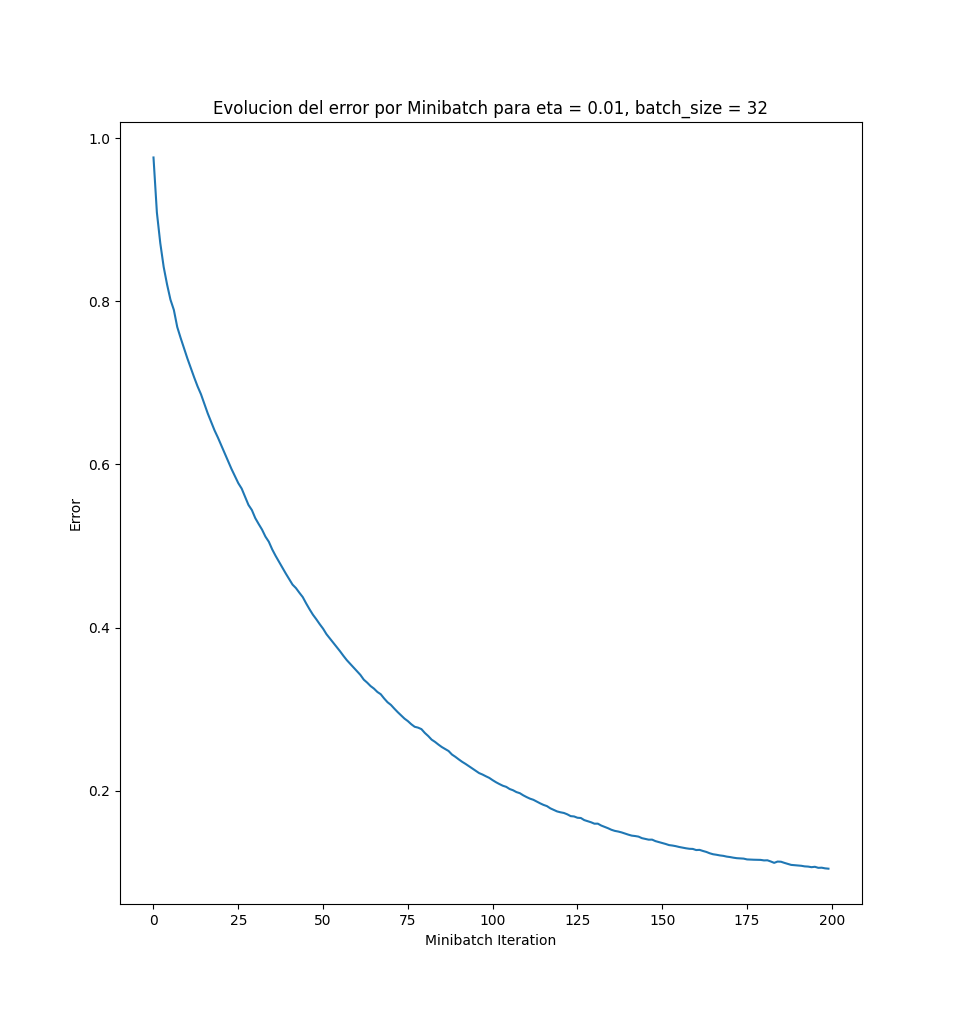
\includegraphics[scale=0.55]{MinibatchError01}

Notar que hay iteraciones en las que el error asciende en vez de descender de forma monótona, como buscábamos en Batch Gradient Descent. Sin embargo, ahora este comportamiento no es indeseable como lo era antes. Para empezar, el ascenso del error es pequeño, no como en Batch Gradient Descent en los que teníamos picos demasiado bruscos. Además, la tendencia general es claramente descendente. Y en ocasiones puede ser interesante poder tener iteraciones que aumenten el error. Ya en el ejercicio 1 nos habría venido bien, tanto para salir de esos pequeños baches como para caernos de un punto de silla hacia un mínimo local.

Estos pequeños aumentos del error se deben a que, como no estamos usando toda la información de la muestra de datos, ciertas iteraciones pueden ir en una dirección confundida que indica el cálculo del gradiente con ese \emph{subset} de los datos.

También puede parecer que las doscientas iteraciones se quedan cortas a la hora de seguir disminuyendo el error. Así que pruebo a poner un máximo de 400 iteraciones para ver si se puede seguir disminuyendo el valor del error, obteniendo la gráfica siguiente:

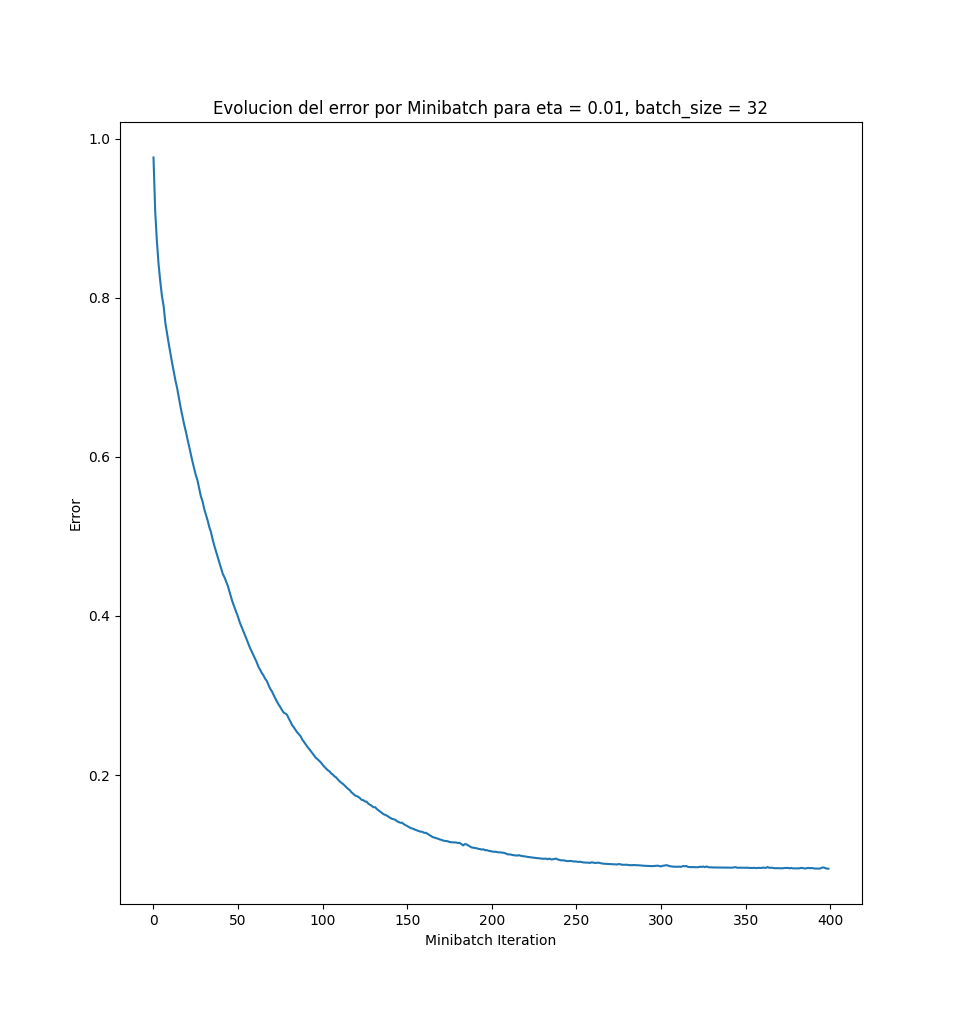
\includegraphics[scale=0.55]{MinibatchError02}

Podemos ver que a partir de las doscientas iteraciones apenas se reduce el error. Alcanzamos una cota para el error que podemos minimizar. Esto puede ser bien porque los datos con los que trabajamos no permiten reducir más el error (hemos alcanzado un mínimo local), o porque a partir de las doscientas iteraciones convendría emplear un $learning\_rate$ más bajo para poder mejorar el error con más precisión.

\pagebreak

\subsection{Apartado 2}

Usamos la función de generación de datos \lstinline{simula_unif(N, 2, size)} que nos devuelve $N$ coordenadas bidimesionales en el cuadrado $[-size, size]^2$

\subsubsection{Subapartado a}

Usando la anterior función generamos los 1000 puntos en el cuadrado $[-1, 1]^2$ usando \lstinline{simula_unif(1000, 2, 1)}, y generamos el siguiente gráfico:

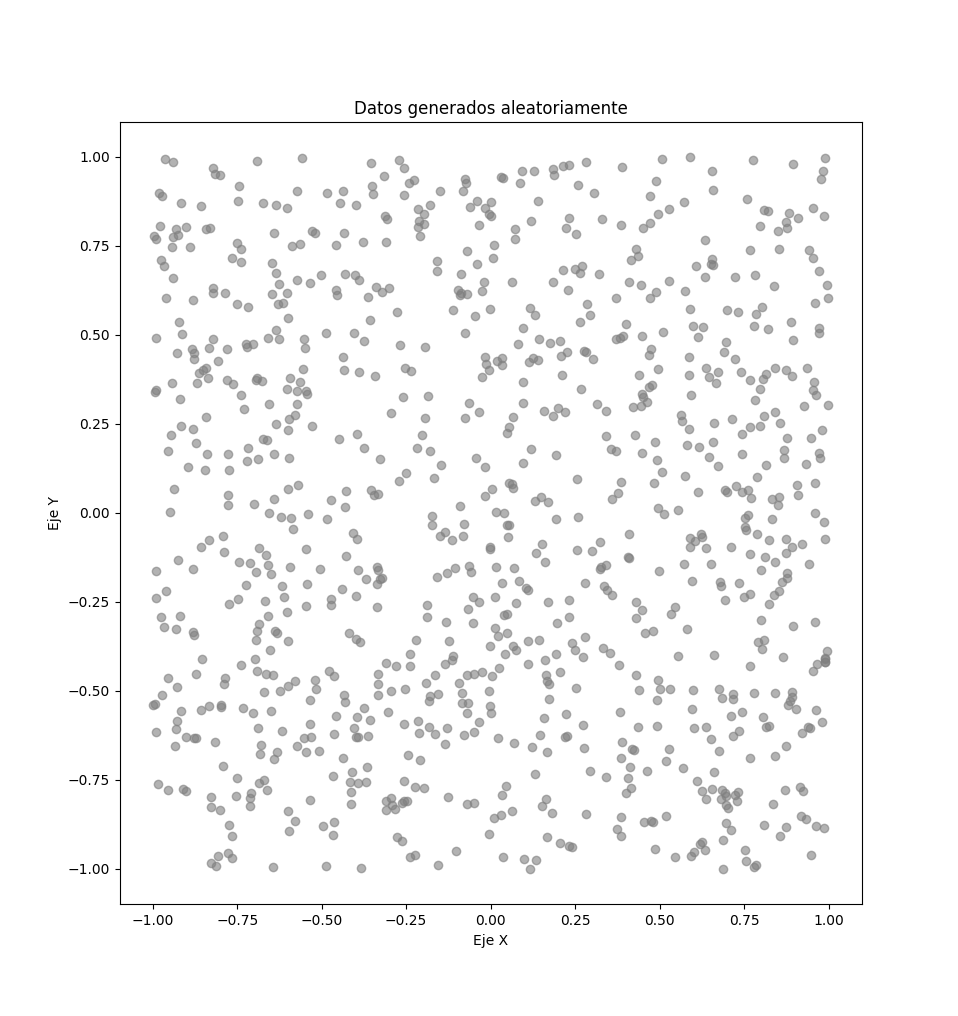
\includegraphics[scale=0.45]{RandomScatterPlot}

\subsubsection{Subapartartado b}

Consideramos la función $f(x_1, x_2) = sign((x_1 - 0.2)^2 + x_2^2 - 0.6)$. Usamos dicha función para etiquetar los datos. Introducimos ruido sobre el 10\% de las etiquetas, es decir, cambiamos el signo del 10\% de las etiquetas. Para ello, generamos los índices $\{0, 1, \ldots, 999\}$, los mezclamos y cambiamos el signo de los datos datos correspondientes a los primeros 100 indices. Por tener más generalidad, trabajamos con el 10\% de los indices generados. Así obtenemos la siguiente gráfica:

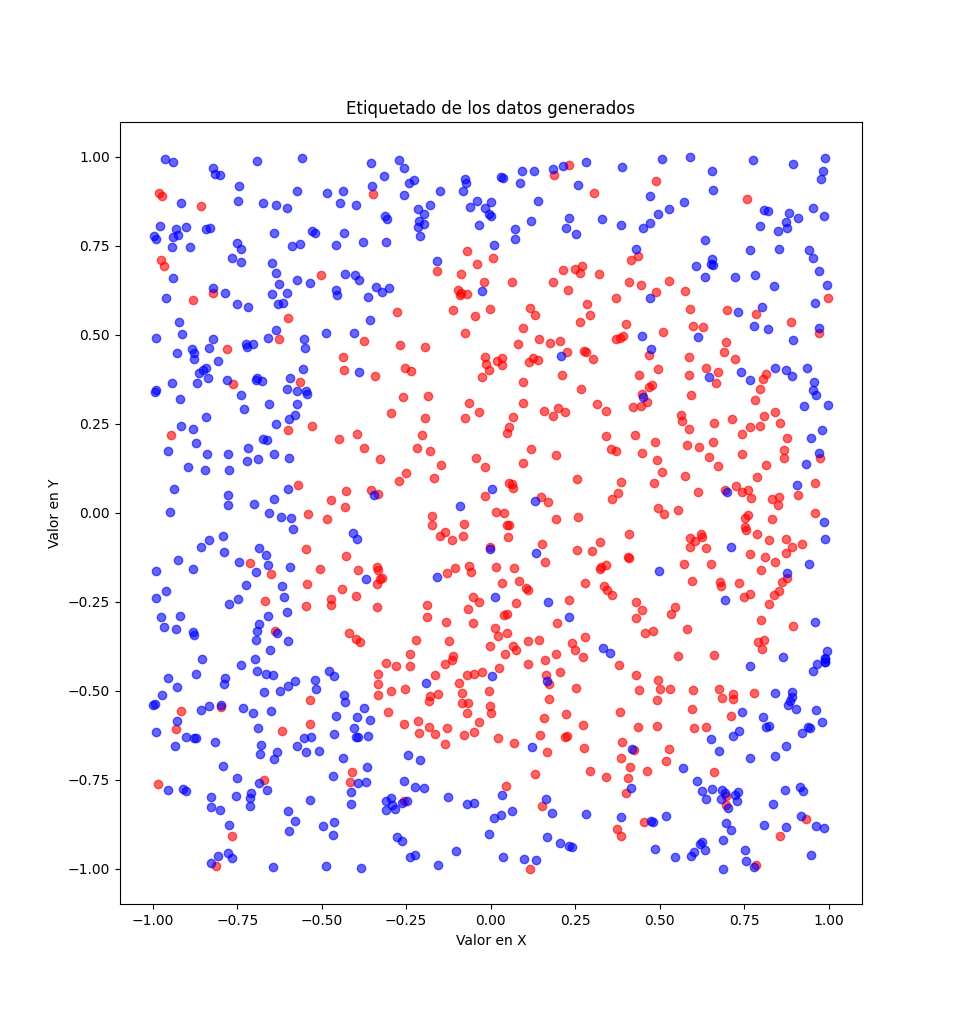
\includegraphics[scale=0.45]{LabeledScatterPlot}

\subsubsection{Subapartartado c}

Ajustamos un modelo lineal usando el vector de características $(1, x_1, x_2)$ usando Gradiente Descendiente Estocástico.

Necesitamos añadir una columna de unos a la matriz de datos generadas. Para ello usamos las instrucciones:

\begin{lstlisting}[language=Python]
number_of_rows = int(np.shape(X)[0])
new_column = np.ones(number_of_rows)
X = np.insert(X, 0, new_column, axis = 1)
\end{lstlisting}

Para lanzar \emph{SGD} establecemos los siguientes parámetros:

\begin{itemize}
    \item Solución inicial: vector de ceros con la dimensionalidad adecuada
    \item $batch\_size$: 32, por lo bien que nos ha funcionado en el ejercicio anterior
    \item Número máximo de iteraciones: 200, el profesor nos comentó que deberían ser suficientes. Y en el apartado anterior vemos que con más iteraciones no mejoramos demasiado el resultado
    \item $\eta$: 0.01 pues hemos explorado otros valores para este problema y este nos ha funcionado bien
\end{itemize}

El algoritmo nos devuelve el siguiente resultado:

\begin{lstlisting}
Los pesos obtenidos son: [ 0.0495547  -0.3450253   0.03473961]
El error de clasficacion en la muestra Ein es: 61.57961277110754
El error cuadratico medio en la muestra Ein es: 0.9290128091406921
El error porcentual en la muestra Ein es: 39.800000000000004%
\end{lstlisting}

Fallamos en prácticamente el 40\% de los datos. Por tanto, no estamos consiguiendo buenos resultados. En este caso, podemos afirmar que los datos no son buenamente tratables con regresión lineal, al menos con el vector de características que estamos trabajando. Esto ya lo podíamos saber fácilmente viendo la función que hemos usado para etiquetar los datos.

Mostramos cómo avanza el error sobre las iteraciones en el minibatch:

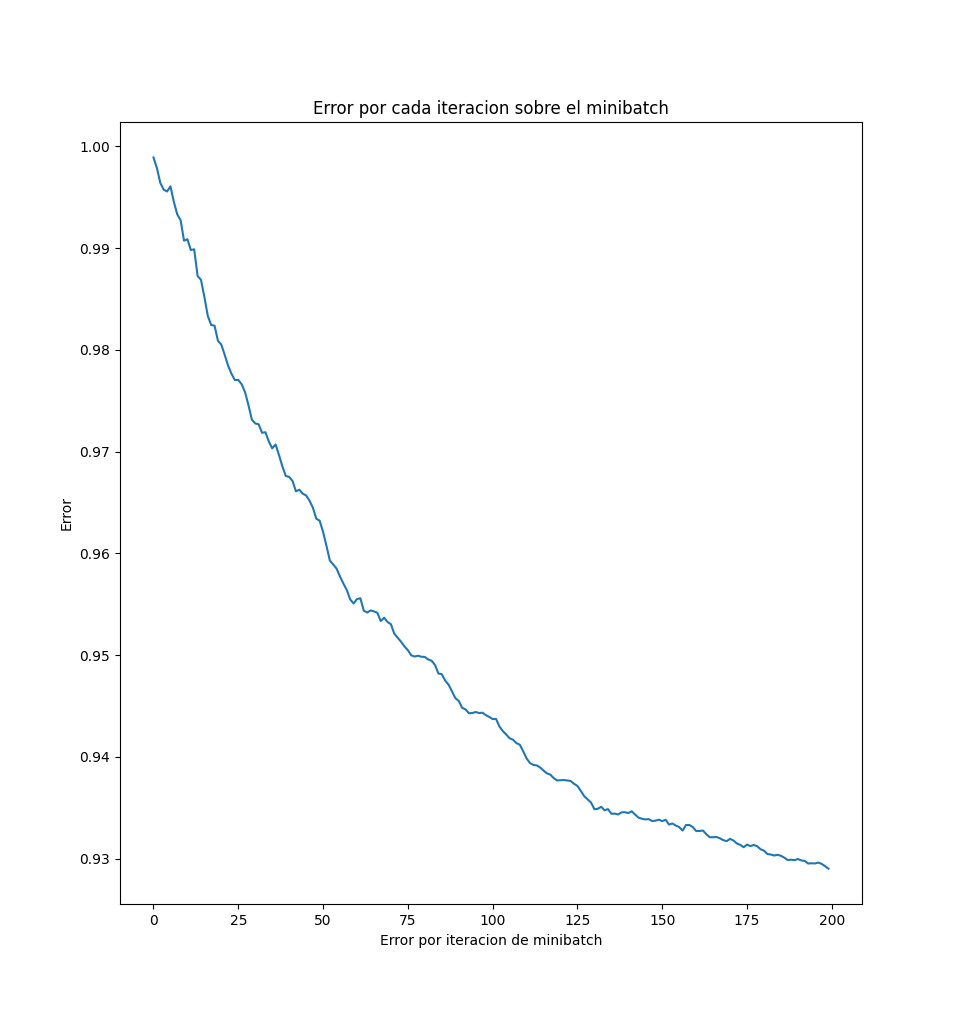
\includegraphics[scale=0.55]{MinibatchError03}

Como en el apartado anterior, vemos que con 200 iteraciones la tendencia de la gráfica es a aplanarse, por lo tanto, con unos resultados tan malos no merece la pena estudiar si con más iteraciones mejoraríamos el resultado.

Y los puntos en los que falla la clasificación:

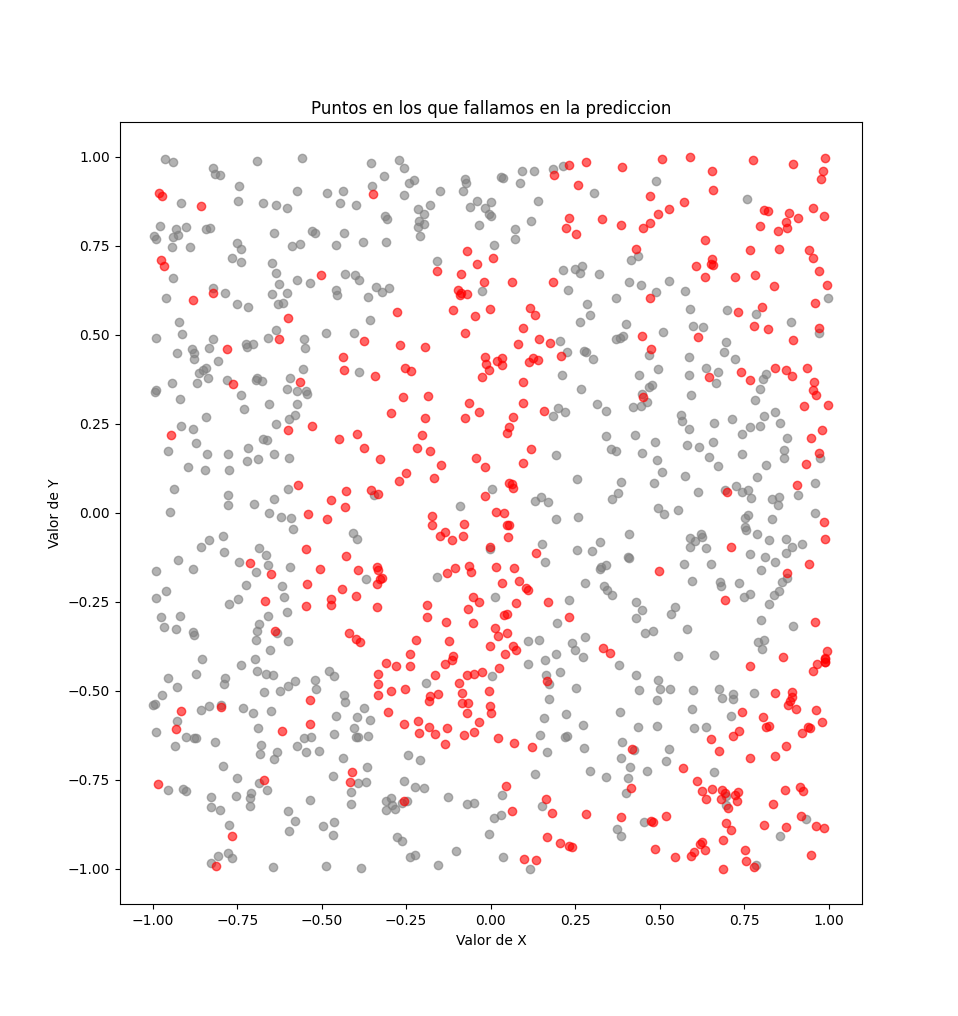
\includegraphics[scale=0.55]{BadPoints05}

\subsubsection{Subapartado d}

Repetimos el experimento 1000 veces. En cada una de estas repeticiones, generamos una nueva muestra aleatoria de 1000 puntos para el training, y otra muestra aleatorioa de 1000 puntos para testing, así que ahora podremos computar el valor tanto de $E\_in$ como de $E\_out$. Los resultados obtenidos son:

\begin{lstlisting}
Error medio porcentual DENTRO de la muestra: 40.41820000000005%
Error medio porcentual FUERA de la muestra: 40.74019999999995%
Error medio cuadratico medio DENTRO de la muestra: 0.9310675034757584
Error medio cuadratico medio FUERA de la muestra: 0.9363078116801644
\end{lstlisting}

Así que repitiendo mil veces el experimento, vemos que la clasificación usando regresión lineal es muy mala. Además, se clasifica prácticamente igual de mal dentro de la muestra de entrenamiento como en la muestra de testing.

\subsubsection{Subapartado e}

Por tanto, como ya hemos comentado, no es adecuado el uso de regresión lineal para clasificar este conjunto de datos. Un 40\% de error no es admisible a la hora de clasificar los datos. Esto era previsible desde el momento que hemos usado una función de etiquetado $f(x,y)$ no lineal, pero un vector de características lineal.

Todo esto es motivación suficiente para emplear el vector de características no lineales del siguiente ejercicio.


\end{document}
